\documentclass{beamer}
\usepackage{beamerthemesplit}
\usetheme{SPbGU}
%{CambridgeUS}
% Выпишем часть возможных стилей, некоторые из них могут содержать
% дополнительные опции
% Darmstadt, Ilmenau, CambridgeUS, default, Bergen, Madrid, AnnArbor,Pittsburg, Rochester,
% Antiles, Montpellier, Berkley, Berlin
\usepackage{pdfpages}
\usepackage{amsmath}
\usepackage{cmap} % for serchable pdf's
\usepackage[T2A]{fontenc} 
\usepackage[utf8]{inputenc}
\usepackage[english,russian]{babel}
\usepackage{indentfirst}
\usepackage{amsmath}
%\usepackage{dot2texi}
\usepackage{tikz}


\usepackage[noend]{algpseudocode}
\usepackage{algorithm}
\usepackage{algorithmicx}
%\usepackage{mathspec}

\usetikzlibrary{shapes,arrows}
\usepackage{fancyvrb}
% Если у вас есть логотип вашей кафедры, факультета или университета, то
% его можно включить в презентацию.

%\usefoottemplate{\vbox{}}%  \tinycolouredline{structure!25}% {\color{white}\textbf{\insertshortauthor\hfill% \insertshortinstitute}}% \tinycolouredline{structure}% {\color{white}\textbf{\insertshorttitle}\hfill}% }}

%\logo{
\includegraphics[width=1cm]{SPbGU_Logo.png}}

%[GLR-анализатор]
\title[]{Cинтаксический анализ динамически формируемых строковых выражений}
%\subtitle[студроект]{Студенческий проект}
\institute[СПбГУ]{
Санкт-Петербургский государственный университет \\
Математико-Механический факультет \\
Кафедра системного программирования }
%[Лукичёв А.С. Григорьев С.В.]


\author[Григорьев Семён]{Григорьев Семён Вячеславович \\
  \and  
  {\bfseries Научный руководитель:} кандидат физико-математических наук, доцент Д.В. Кознов \\ 
%  \and
%  {\bfseries Рецензент:} д.ф.-м.н., проф. Б.К. Мартыненко  
}

\date{2015г.}

\definecolor{orange}{RGB}{179,36,31}

\begin{document}
{

\begin{frame}
\begin{center}
{
\includegraphics[width=1cm]{SPbGU_Logo.png}}
\end{center}
\titlepage
\end{frame}
}

\begin{frame}[fragile]
    \transwipe[direction=90]
    \frametitle{Динамически формируемые строковые выражения: пример}
    \begin{itemize}
        \item Встроенный SQL
\begin{Verbatim}[commandchars=\\\{\}]
\textcolor{blue}{let} p cond fldLst =
    \textcolor{blue}{let mutable} flds = \textcolor{orange}{"id"}
    \textcolor{blue}{for} fld \textcolor{blue}{in} fldLst \textcolor{blue}{do}
        flds <- flds + \textcolor{orange}{", "} + fld 
    \textcolor{blue}{let} tbl = \textcolor{blue}{if} cond \textcolor{blue}{then} \textcolor{orange}{"table1"} \textcolor{blue}{else} \textcolor{orange}{"table2"}    
    \underline{execute} (\textcolor{orange}{"SELECT"} + flds + \textcolor{orange}{"FROM"} + tbl)
\end{Verbatim}
        \item JavaScript в Java
\begin{Verbatim}[commandchars=\\\{\}]
\textcolor{blue}{String} script =
    \textcolor{orange}{"function hello(name) { print(’Hello, ’ + name); }"};
engine.eval(script);
\textcolor{blue}{Invocable} inv = (\textcolor{blue}{Invocable}) engine;
inv.invokeFunction(\textcolor{orange}{"hello"}, \textcolor{orange}{"Scripting!!!"} );
\end{Verbatim}
    \end{itemize}

\end{frame}

\begin{frame}
    \transwipe[direction=90]
    \frametitle{Динамически формируемые строковые выражения: проблемы}
    \begin{itemize}
        \item Значение выражения --- код на некотором языке и его нужно соответствующим образом поддерживать и обрабатывать
        \item Однако для стандартных инструментов это просто строки
        \begin{itemize}
            \item Ошибки в динамически формируемых выражениях обнаруживаются лишь во время выполнения
            \item Нет поддержки в средах разработки
            \item Затруднён реинжиниринг ПО, разработанного с использованием встроенных языков                
        \end{itemize}
        \item Существует множество различных языков и задач
    \end{itemize}
\end{frame}

\begin{frame}
    \transwipe[direction=90]
    \frametitle{Обзор}
    \begin{itemize}
        \item Построение аппроксимации $L_R \rightarrow $ \ проверка включения $L_{R} \subseteq L(G)$, $G$ -- КС грамматика референсного языка 
        \begin{itemize}
            \item JSA, PHPSA
        \end{itemize}
        \item Alvor -- построение регулярной аппроксимации  $ \rightarrow $ \ лексический анализ $ \rightarrow $ \ синтаксический анализ
        \item Kyung-Goo Doh -- data-flow уравнения + LALR(1) анализ + абстрактная интерпретация стеков + атрибутные грамматики
        \item Для работы с сематникой нужно иметь лес вывода -- множество деревьев для всех $\omega \in L_R$ выводимых в G
    \end{itemize}
\end{frame}

\begin{frame}
    \transwipe[direction=90]
    \frametitle{Цели и задачи работы}
    \begin{itemize}
        \item Создать подход к статическому синтаксическому анализу динамически формируемых выражений, позволяющего обрабатывать произвольную регулярную аппроксимацию без потери точности.
        \begin{itemize}
            \item Обработка регулярной аппроксимации
            \item Построение леса вывода
        \end{itemize}
        \item Разработать технологию для создания инструментов статического анализа встроенных текстовых языков, реализующей данный алгоритм.
    \end{itemize}
\end{frame}

\begin{frame}
    \transwipe[direction=90]
    \frametitle{Положения, выносимые на защиту}
        \begin{itemize}
            \item Разработан алгоритм синтаксического анализа динамически формируемых выражений, позволяющий обрабатывать произвольную регулярную аппроксимацию множества значений выражения в точке выполнения, реализующий эффективное управление стеком и гарантирующий конечность представления леса вывода. Доказана завершаемость и корректность предложенного алгоритма.
            \item Создана архитектура инструментария для разработки программных средств синтаксического анализа динамически формируемых строковых выражений.
            \item Разработана методика анализа динамически формируемых строковых выражений в проектах по реинжинирингу информационных систем.  
        \end{itemize}
\end{frame}

\begin{frame}
    \transwipe[direction=90]
    \frametitle{Научная новизна}
    \begin{itemize}
        \item Предложенный алгоритм предназначен для синтаксического анализа динамически формируемых выражений и построения компактной структуры данных, содержащей для всех корректных значений выражения их деревья вывода.
        \item Предложена архитектура инструментального средства, позволяющего упростить создание новых инструментов для анализа динамически формируемых выражений на любых языках программирования.
    \end{itemize}
\end{frame}

\begin{frame}
    \transwipe[direction=90]
    \frametitle{Архитектура: цели и задачи}
    \begin{itemize}
        \item Упростить создание инструментов анализа динамически формируемых выражений
        \item Необходимв: набор готовых компонентов, генераторы лексических и синтаксических анализаторов
    \end{itemize}
\end{frame}

\begin{frame}
    \transwipe[direction=90]
    \frametitle{Архитектура: процесс анализа}
    \begin{center}
        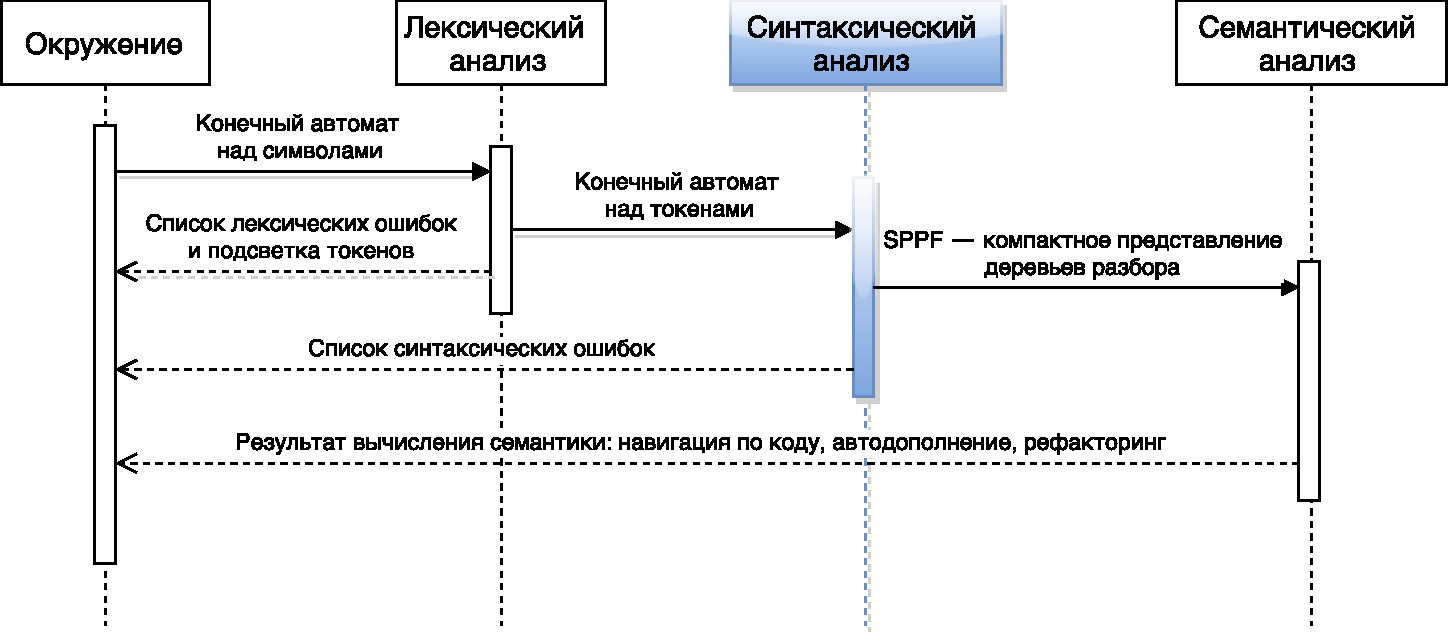
\includegraphics[width=300pt]{pictures/Seq.pdf}
    \end{center}
\end{frame}

\begin{frame}
    \transwipe[direction=90]
    \frametitle{Архитектура: инструментарий}
    \begin{center}
        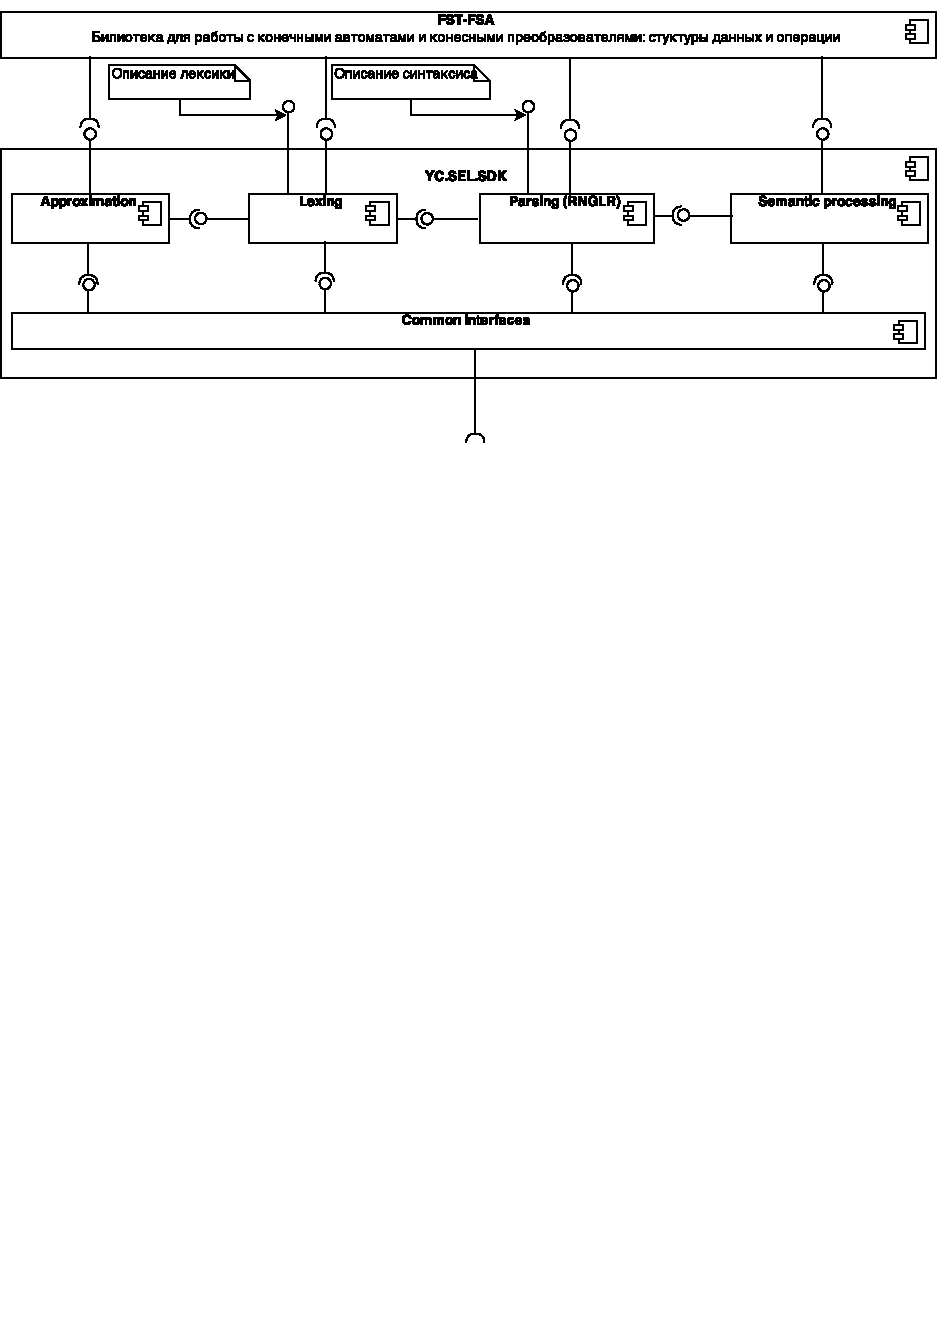
\includegraphics[width=300pt]{pictures/Components.pdf}
    \end{center}
\end{frame}

\begin{frame}
    \transwipe[direction=90]
    \frametitle{Аппроксимация и лексический анализ}    
\end{frame}

\begin{frame}
    \transwipe[direction=90]
    \frametitle{Синтаксический анализ: постановка задачи}
    \begin{itemize}    
        \item $G=\langle N,\Sigma, P,S\rangle$ -- однозначная КС грамматика
        \item $R$ -- регулярное множество над алфавитом ${\Sigma}^{'} \subseteq \Sigma $
        \item $AST(t,\omega,G)$ -- является ли $t$ деревом вывода $\omega$ в грамматике $G$
    \end{itemize}
    Необходимо построить алгоритм $\mathbb{P}$ такой что
    $(\forall \omega \in R) (\omega \in L(G) \Rightarrow (\exists t \in \mathbb{P}(R,G))AST(t, \omega, G))$
    $\land (\forall t \in \mathbb{P}(R,G))(\exists s \in R)AST(t,\omega,G)$
\end{frame}

\begin{frame}
    \transwipe[direction=90]
    \frametitle{Синтакический анализ: идеи алгоритма}
    \begin{itemize}         
        \item Основан на RNGLR алгоритме
        \item Вход: КА
    \end{itemize}
\end{frame}

\begin{frame}
    \transwipe[direction=90]
    \frametitle{Синтакический анализ: идеи алгоритма}


The general idea of the algorithm is to traverse the automaton graph and sequentially construct GSS, similarly as in RNGLR.
However, as we deal with a graph instead of a linear stream, the next symbol turns into the \emph{set of terminals} on 
all outgoing edges of current vertex. This results in a different semantics of pushing and reducing (see line~5, 
Algorithm~\ref{processVertex}, and lines~9 and~21, Algorithm~\ref{gss_construction}). We use queue $\mathcal Q$ to control the 
order of automaton graph vertices processing. Every time a new GSS vertex is added, all zero-reductions have to be performed 
and then new tokens have to be shifted, so a corresponding graph vertex has to be enqueueed for further processing. 
Addition of new GSS edge can produce reductions to handle, so the graph vertex at the tail of the added edge has 
also to be enqueueed (see Algorithm~\ref{gss_construction}). Reductions are applied along the paths in GSS, and if we add
a new edge to some tail vertex, which was already presented in GSS, we also have to recalculate all \emph{passing} reductions
(see \emph{applyPassingReductions} function in Algorithm~\ref{processVertex}).
\end{frame}

\begin{frame}
    \transwipe[direction=90]
    \frametitle{Синтакический анализ: идеи алгоритма}


Besides parser $state$ and $level$ (which is equal to the input automaton state), 
a collection of \emph{passing reductions} is stored in a GSS vertex. Passing reduction is a 
triplet $(startV, N, l)$, representing reductions, whose path contains given GSS vertex. 
This triplet is similar to one describing reduction, where $l$ is a remaining length of the path. 
Passing reductions are stored for every vertex of the path (except for the first and the last) 
during path search in \emph{makeReductions} function (see Algorithm~\ref{processVertex}).

We inherit SPPF construction from the original RNGLR; in our case, 
derivation trees for strings, accumulated along the paths of the input automaton 
graph, are merged. 
\end{frame}


\begin{frame}
    \transwipe[direction=90]
    \frametitle{Синтакический анализ: идеи алгоритма}

Likewise RNGLR, we associate GSS vertices with positions in the input,
and, in our case, a position coincides with some state of input automaton. We construct some
inner data structure (referred to as \emph{inner graph}) by copying input automaton graph and 
extending each its vertex with the following collections: 

\begin{itemize}
  \item \emph{processed}: GSS vertices, for which all the pushes were processed. 
   This set aggregates all GSS vertices, associated with inner graph vertex.
  \item \emph{unprocessed}: GSS vertices, for which all the pushes are to be processed. 
   This set is analogous to $\mathcal{Q}$ of original RNGLR.
  \item \emph{reductions}: a queue, which is analogous to $\mathcal{R}$ of original RNGLR: 
   all reductions to be processed.
  \item \emph{passingReductionsToHandle}: pairs of GSS vertex and GSS edge to apply 
   passing reductions along them.
\end{itemize}
\end{frame}

\begin{frame}
    \transwipe[direction=90]
    \frametitle{Алгоритм: завершаемость}
    \begin{theorem}
             Algorithm terminates for any input.
    \end{theorem}

    \begin{proof}
       Each vertex of inner representation of the input finite automaton contains, at most, $N$ GSS vertices, where $N$ is a number of parser states. So, the total number of 
       GSS vertices is, at most, $N\times n$, where $n$ is the number of vertices in the inner graph. 
       Since GSS has no multi-edges, the number of its edges is $O((N\times n)^2)$. The algorithm 
       dequeues vertex to be processed from $\mathcal Q$ in the each iteration of the 
       main loop. Vertices are enqueued to $\mathcal Q$ only when a new edge is added to GSS. Since the number of GSS edges is finite, the algorithm always terminates.
    \end{proof}

\end{frame}

\begin{frame}
    \transwipe[direction=90]
    \frametitle{Алгоритм: завершаемость}
    \begin{definition}
         \emph{Correct tree} is an ordered tree with the following properties:
        \begin{enumerate}
            \item The root is the start nonterminal of the grammar $G$.
            \item The leaf nodes are terminals of $G$. The sequence of the leaf nodes corresponds to some path in the inner graph. 
            \item The interior nodes are nonterminals of $G$. All children of nonterminal $N$ correspond to the symbols of the right-hand side of some production for $N$ in $G$.
        \end{enumerate}
    \end{definition}
\end{frame}

\begin{frame}
    \transwipe[direction=90]
    \frametitle{Алгоритм: корректность}
        \begin{lemma}[Lemma 1]
    For every GSS edge $(v_{t}, v_{h})$, $v_{t} \in V_{t}.processed$, $v_{h} \in V_{h}.processed$, the terminals of the associated subtree correspond to some path in the inner graph $p$ 
from $V_{h}$ to $V_{t}$.
    \end{lemma}

    \begin{proof}
        The proof is by induction on the height of derivation tree.
    \end{proof}

\end{frame}

\begin{frame}
    \transwipe[direction=90]
    \frametitle{Алгоритм: корректность}
    \begin{theorem}
       Every generated from SPPF tree is correct.
    \end{theorem}

    \begin{proof}
      Consider arbitrary tree, generated from SPPF, and prove that it is correct. The first and the third statements
of correctness definition immediately follow from SPPF definition. 

\textsc{Lemma 1} proves the second item of the definition by consideration of all the edges from the GSS vertex
on the last level having accepting state to the vertex on the 0-level with the start parser state.

    \end{proof}

\end{frame}

\begin{frame}
    \transwipe[direction=90]
    \frametitle{Алгоритм: корректность}
    \begin{theorem}
       \textit{For every path $p$ in the inner graph, recognized w.r.t. reference grammar, a correct tree corresponding to $p$ can 
be generated from SPPF.}

    \end{theorem}

    \begin{proof}
Consider arbitrary correct tree and show it can be generated from SPPF. The proof follows the proof of correctness 
for RNGLR algorithm, except for the following moment. RNGLR constructs GSS layer-by-layer: it is guaranteed, that $\forall j \in [0..i-1]$ 
$j$-th level of the GSS would be fixed by the time, when $i$-th level is processed. In our case, 
this property does not hold, which leads to a possible generation of some paths for already applied reductions. 
The only possible way to actually add a new path is to add an edge $(v_{t}, v_{h})$, where $v_{t}$ is already in the GSS and 
it has some incoming edges. Since the algorithm stores which reductions have passed through each vertex, to overcome this problem 
it is sufficient to continue passing reductions, stored in $v_{t}$, and this is exactly what \emph{applyPassingReductions} 
function does. 
    \end{proof}

\end{frame}


\begin{frame}
    \transwipe[direction=90]
    \frametitle{Алгоритм: пример работы}
\end{frame}

\begin{frame}[t]
    \transwipe[direction=90]
    \frametitle{Методология}
    \begin{itemize}
        \item  Берём и генерируем
    \end{itemize}
\end{frame}

\begin{frame}[t]
    \transwipe[direction=90]
    \frametitle{Апробация: синтетические замеры}
\end{frame}

\begin{frame}[t]
    \transwipe[direction=90]
    \frametitle{Апробация: трансляция динамического SQL}
\end{frame}

\begin{frame}[t]
    \transwipe[direction=90]
    \frametitle{Апробация: плагин к ReSharper}
\end{frame}

\begin{frame}
    \transwipe[direction=90]
    \frametitle{Публикации}
  \begin{itemize}
      \item Кириленко Я.А., Григорьев С. В., Авдюхин Д. А. Разработка синтаксических анализаторов в проектах по автоматизированному реинжинирингу информационных систем.  Научно-технические ведомости Санкт-Петербургского государственного политехнического университета информатика, телекоммуникации, управление. Т. 3, N 174, 2013. C. 94 --- 98.
      \item Григорьев С. В., Вербицкая Е. А., Полубелова М. И., Иванов А. В., Мавчун Е. В. Инструментальная поддержка встроенных языков в интегрированных средах разработки. Моделирование и анализ информационных систем. Т. 21, N 6, 2014. С. 131---143.
      \item Григорьев С.В. Алгоритм синтаксического анализа динамически формируемых выражений.
  \end{itemize} 
\end{frame}

\begin{frame}
    \transwipe[direction=90]
    \frametitle{Публикации}
  \begin{itemize}
          \item Semen Grigorev, Iakov Kirilenko. GLR-based abstract parsing. In Proceedings of the 9th Central \& Eastern European Software Engineering Conference in Russia (CEE-SECR ’13). 2013. ACM, New York, NY, USA. 1-9 p.
          \item Semen Grigorev, Ekaterina Verbitskaia, Andrei Ivanov, Marina Polubelova, Ekaterina Mavchun. String-embedded language support in integrated development environment. In Proceedings of the 10th Central and Eastern European Software Engineering Conference in Russia (CEE-SECR '14). 2014. ACM, New York, NY, USA. 1-11 p.
          \item Semen Grigorev, Iakov Kirilenko. From Abstract Parsing to Abstract Translation. Proceedings of the Spring/Summer Young Researchers' Colloquium on Software Engineering. 2014. Saint Petersburg, Russia. 1-5 p.
  \end{itemize} 
\end{frame}

\begin{frame}[fragile] 
    \transwipe[direction=90]
    \frametitle{Алгоритм: псевдокод}
\begin{algorithmic}[1]
\Function{parse}{$grammar, automaton$}
  \State{$inputGraph \gets$ construct inner graph representation of $automaton$}
  \State{$parserSource \gets$ generate RNGLR parser tables for $grammar$}
  \If{$inputGraph$ contains no edges}
    \If{$parserSource$ accepts empty input} {report success}
    \Else { report failure}
    \EndIf
  \Else
    \State{\Call{addVertex}{$inputGraph.startVertex, startState$}}
    \State{$\mathcal{Q}.Enqueue(inputGraph.startVertex)$}
    \While{$Q$ is not empty}
      \State{$v \gets \mathcal{Q}.Dequeue()$}
      \State{\Call{makeReductions}{$v$}}
      \State{\Call{push}{$v$}}
      \State{\Call{applyPassingReductions}{$v$}}
    \EndWhile
    \If{$v_f.level = q_f$ and $v_f.state$ is accepting} {report success}
    \Else { report failure}
    \EndIf
  \EndIf
\EndFunction
\end{algorithmic}
\end{frame}

\begin{frame}[fragile] 
    \transwipe[direction=90]
    \frametitle{Алгоритм: псевдокод}
\begin{algorithmic}[1]
%\caption{Single vertex processing}
%\label{processVertex}

\Function{makeReductions}{$innerGraphV$}
  \While{$innerGraphV.reductions$ is not empty}
    \State{$(startV, N, l) \gets innerGraphV.reductions.Dequeue()$}
    \State{find the set of vertices $\mathcal{X}$ reachable from $startV$}
    \State{    along the path of length ($l-1$), or $0$ if $l=0$;}
    \State{add $(startV, N, l-i)$ in $v.passingReductions$,}
    \State{    where $v$ is an $i$-th vertex of the path}
    \ForAll{$v_{h}$ in $\mathcal{X}$}
      \State{$state_{t} \gets$ calculate new state by $v_{h}.state$ and nonterminal $N$}
      \State{\Call{addEdge}{$v_{h}, startV, state_{t}, (l=0)$}}
    \EndFor
  \EndWhile
\EndFunction
\end{algorithmic}
\end{frame}


\begin{frame}[fragile] 
    \transwipe[direction=90]
    \frametitle{Алгоритм: псевдокод}
\begin{algorithmic}[1]

\Function{push}{$innerGraphV$}
  \State{$\mathcal{U} \gets$ copy $innerGraphV.unprocessed$}
  \State{clear $innerGraphV.unprocessed$}
  \ForAll{$v_{h}$ in $\mathcal{U}$}  
    \ForAll{$e$ in outgoing edges of $innerGraphV$}
      \State{$push \gets$ calculate next state by $v_{h}.state$ and the token on $e$}
      \State{\Call{addEdge}{$v_{h}, e.Head, push, false$}}
      \State{add $v_{h}$ in $innerGraphV.processed$}
    \EndFor
  \EndFor
\EndFunction

\Function{applyPassingReductions}{$innerGraphV$}
  \ForAll{$(v, edge)$ in $innerGraphV.passingReductionsToHandle$}
    \ForAll{$(startV, N, l) \gets v.passingReductions.Dequeue()$}
      \State{find the set of vertices $\mathcal{X}$,}
      \State{    reachable from $edge$ along the path of length ($l-1$)}
      \ForAll{$v_{h}$ in $\mathcal{X}$}
        \State{$state_{t} \gets$ calculate new state by $v_{h}.state$ and nonterminal $N$}
        \State{\Call{addEdge}{$v_{h}, startV, state_{t}, false$}}
      \EndFor
    \EndFor
  \EndFor
\EndFunction
\end{algorithmic}
\end{frame}

\begin{frame}[fragile] 
    \transwipe[direction=90]
    \frametitle{Алгоритм: псевдокод}
\begin{algorithmic}[1]
%\caption{GSS construction}
%\label{gss_construction}
\Function{addVertex}{$innerGraphV, state$}
  \State{$v \gets$ find a vertex with state $=state$ in}
  \State{    $innerGraphV.processed \cup innerGraphV.unprocessed$}
  \If{$v$ is not $null$ } \Comment{The vertex have been found in GSS}
    \State{\Return{($v, false$)}} 
  \Else
    \State{$v \gets$ create new vertex for $innerGraphV$ with state $state$}
    \State{add $v$ in $innerGraphV.unprocessed$}
    \ForAll{$e$ in outgoing edges of $innerGraphV$}
      \State{calculate the set of zero-reductions by $v$}
      \State{    and the token on $e$ and add them in $innerGraphV.reductions$}
    \EndFor
    \State{\Return{$(v, true$)}}
  \EndIf
\EndFunction
\end{algorithmic}
\end{frame}

\begin{frame}[fragile] 
    \transwipe[direction=90]
    \frametitle{Алгоритм: псевдокод}
\begin{algorithmic}[1]
\Function{addEdge}{$v_{h}, innerGraphV, state_{t}, isZeroReduction$}
  \State{$(v_{t}, isNew) \gets$ \Call{addVertex}{$innerGraphV, state_{t}$}}
  \If{GSS does not contain edge from $v_{t}$ to $v_{h}$}
    \State{$edge \gets$ create new edge from $v_{t}$ to $v_{h}$}
    \State{$\mathcal{Q}.Enqueue(innerGraphV)$}
    \If{not $isNew$ and $v_{t}.passingReductions.Count>0$}
      \State{add $(v_{t}, edge)$ in $innerGraphV.passingReductionsToHandle$}
    \EndIf
    \If{not $isZeroReduction$}
      \ForAll{$e$ in outgoing edges of $innerGraphV$}
        \State{calculate the set of reductions by $v$}
        \State{    and the token on $e$ and add them in $innerGraphV.reductions$}
      \EndFor
    \EndIf
  \EndIf
\EndFunction
\end{algorithmic}
\end{frame}



\end{document}
